\makeatletter
\def\input@path{{../}}
\makeatother
\documentclass[../master_thesis.tex]{subfiles}
\begin{document}
\chapter{Quantum Chemistry}
\section{\ac{QM}}

\subsection{The Postulates of \ac{QM}}

\ac{QM} are based on a set rules that define operations and states. We will
present these rules as six different postulates of \ac{QM} (sometimes divided
as 5) \cite{Atkins:2011, Cohen:1973}.

\subsubsection{First Postulate}
The first postulate states that everything we can know about a physical system
can be extracted from the wave function $\Psi(x, t)$ of that system
\cite{Atkins:2011}. Additionally at a time $t_0$ the system is defined by
a state vector (or wave function) $\ket{\Psi(t_0)}\in L^2$ that has a defined
finite scalar product as \cite{Cohen:1973}:
\begin{equation}
  \braket{\Psi|\Psi} = \|\ket{\Psi}\|^2 =  \int_{\mathbb{R}^3}\Psi^\star\Psi d\vec{r}
\end{equation}

\subsubsection{Second Postulate}
A generic observable $O$ is represented by the application of a generic operator
$\hat{O}$. Two such observables are the position and momentum of a particle. These are
represented by $\hat{q_i}$ and $\hat{p_i}$ respectively, where
$i = \{x, y, z\}$. These operators fulfill the following commutation relations
\cite{Atkins:2011, Cohen:1973}:
\begin{align}
  \begin{split}
    [q_i, p_j] &= i \hbar \delta_{ij}\\
    [q_i, q_j] &= 0 \\
    [p_i, p_j] &= 0
  \end{split}
\end{align}

The operators that represent observables are hermitian, meaning that
\cite{Cohen:1973}:
\begin{equation}
  \hat{O} = (\hat{O}^{\star})^T = (\hat{O}^T)^{\star} = \hat{O}^{\dagger}
\end{equation}

These operators are linear as well:
\begin{equation}
    \hat{O}(f + g) = \hat{O}f + \hat{O}g\label{eq:oplinearity}
\end{equation}
Where $f$ and $g$ are functions.

\subsubsection{Third Postulate}
When measuring an observable $O$ on a system $\ket{\Psi}$, The only possible
values of the observable are eigenvalues of the corresponding operator $\hat{O}$
unto the measured system $\Psi$ at its current state $\ket{\Psi_i}$. The \eivals
are solutions to the following equation \cite{Cohen:1973}
\begin{equation}
  \hat{O}\ket{\Psi_i} = o_i \ket{\Psi_i}
\end{equation}
This holds true even if the state measured is not an eigenstate of $\hat{O}$.

We can represent a system state vector $\ket{\Psi}$ that is not an eigenstate
of $\hat{O}$ as a linear combination of eigenstates $\ket{i}$ of the operator
\begin{equation}
  \ket{\Psi} = \sum_i c_i \ket{i}
\end{equation}
where the coefficients $c_i$ are computed as the projection of $\ket{\Psi}$ onto
the eigenstates of the operator.
\begin{equation}\label{eq:projcoeff}
  c_i = \braket{i|\Psi}
\end{equation}
Let us say that we apply the generic operator on one of its eigenstates that
is multiplied with the projection coefficient $c_i$ from Equation \ref{eq:projcoeff}.
This gives us
\begin{equation}
  \hat{O}c_i\ket{i} = c_i\hat{O}\ket{i} = c_i o_i\ket{i} = o_i c_i\ket{i}
\end{equation}
Which tells  us that $c_i\ket{i}$ is also an eigenstate of $\hat{O}$ with the
same \eival as $\ket{i}$. Since $c_i\ket{i}$ is one of the components in the
eigenstate $\ket{\Psi}$ applying the operator on it will always give us exactly
one of its \eivals, with different probabilities  depending on its projection on the set
of eigenstates of the operator \cite{Cohen:1973}. The fourth postulate will give
us the way to calculate this probability.

\subsubsection{Fourth Postulate}
The fourth postulate states the possible probabilities of getting a specific
\eival for a given measurement.
Let $\ket{\Psi_i}$ be an \eifunc of $\hat{O}$ such that:
\begin{equation}
  \hat{O}\ket{\Psi_i} = o_i\ket{i}
\end{equation}
and
\begin{equation}
  \ket{\Psi} = \sum_i c_i \ket{i} \label{eq:lincomb}
\end{equation}
has no degenerate \eival,
The probability of measuring \eival  $o_i$ from $\ket{\Psi}$ is given by
\cite{Cohen:1973}:
\begin{align} \label{eq:post4}
  \begin{split}
    \mathscr{P}(o_i) &= \abs{\braket{i|\Psi}}^2\\
                     &= \sum_{j}c_i^\star c_j\braket{i|j}\\
                     &= \sum_{j}c_i^\star c_j\delta_{ij}\\
                     &= \abs{c_i}^2
  \end{split}
\end{align}

Following the equation \ref{eq:post4} the probability of measuring the
\eival $o_i$ from $\ket{\Psi_i}$ is just one. The sum of all the probabilities
for each \eival is:
\begin{equation}
  \sum_i\mathscr{P}(o_i) = \sum_i \abs{c_i}^2 = 1
\end{equation}
Here we have ignored the case for degenerate \eival and continuous spectra of
\eival, where the method is analogous to the one used above. The reader is
invited to look them up themselves in \cite{Cohen:1973, Atkins:2011}.

\subsubsection{Fifth Postulate}
The fifth postulate states that immediately after a measurement where the \eival was $o_i$
the state of the system $\ket{\Psi}$ collapses into a state where the only value one
can measure is $o_i$, that is $ \ket{\Psi_i} $ using the conventions stated in postulate 3 and 4.
This is because before measuring, the probabilities for any \eival
is as stated in the fourth postulate. When the value has been measured, though,
the uncertainty does not exists, as the state of the system must be one that gives
exactly that value. The following Equation \ref{eq:post5} represents the postulate.
\begin{equation}\label{eq:post5}
  \ket{\Psi} \stackrel{o_i}{\Rightarrow} \ket{\Psi_i}
\end{equation}

\subsubsection{Sixth Postulate}
The system when undisturbed changes in a deterministic way \cite{Cohen:1973}.
This change is governed by the time dependent \SE \cite{Cohen:1973, Atkins:2011}:
\begin{equation}\label{eq:tdepSE}
  i\hbar\frac{\partial}{\partial t} \ket{\Psi} = \hat{H}\ket{\Psi}
\end{equation}
Where $\tilde{H}$ is the Hamiltonian operator which has the total energy of the
system as its \eivals.

\subsection{The \SE}
Lets consider the following \SE for a particle allowed to move in only one dimension
and where its potential energy varies with position (e.g. the Harmonic oscillator
model \cite{Cohen:1973, Atkins:2014}).
\begin{equation}
  \hat{H}\Psi = \left(-\frac{\hbar^2}{2m}\frac{\partial^2 }{\partial x^2} + \hat{V}(x)\right)\Psi = i\hbar\frac{\partial}{\partial t} \Psi\label{eq:1DSE}
\end{equation}
We can substitute $$\Psi(x, t)=\psi(x)\tau(t)$$ into \ref{eq:1DSE}
by assuming that the wave function can be separated into spatial and time dependent
functions \cite{Atkins:2011}:
\begin{align}
  \begin{split}\label{eq:sepvar1DSE}
    \left(-\frac{\hbar^2}{2m}\frac{\partial^2 }{\partial x^2} + \hat{V}(x)\right)\psi\tau &= i\hbar\frac{\partial}{\partial t} \psi\tau \\
    -\frac{\hbar^2}{2m}\tau\frac{d^2 \psi}{d x^2} + \hat{V}(x)\psi\tau &= i\hbar\psi\frac{d\tau}{d t}\\
    -\frac{\hbar^2}{2m}\frac{1}{\psi}\frac{d^2\psi }{d x^2} + \hat{V}(x) &= i\hbar\frac{1}{\tau}\frac{d\tau}{d t}
  \end{split}
\end{align}
In the last step of the Equation \ref{eq:sepvar1DSE} we divided both sides with $\frac{1}{\tau\psi}$.
This shows us that, since the left-hand side of the equation is only dependent on $x$ and the right-hand
side is only dependent on $t$, no matter how much we change the each of the coordinates, they must always equal to
a constant. This constant will be denoted by $E$ as it is the energy of the system. This gives us the following set of equations \cite{Atkins:2011}:
\begin{subequations}
  \label{eq:sysSE}
  \begin{align}
    -\frac{\hbar^2}{2m}\frac{d^2\psi}{d x^2} + \hat{V}(x)\psi &= E\psi  \label{eq:timeindepWF}\\
    i\hbar\frac{d\tau}{d t} &= E\tau  \label{eq:timedepWF}
  \end{align}
\end{subequations}
Equation \ref{eq:timedepWF} can be solved by observation as \cite{Atkins:2011, Cohen:1973} :
\begin{equation}
  \tau(t) = e^{-iE\frac{t}{\hbar}}
\end{equation}
while the remaining Equation \ref{eq:timeindepWF} can be rewritten as
\begin{equation}
  \hat{H}\psi = E\psi\label{eq:timeindepSE}
\end{equation}
Which is the time-independent \SE.

The energy of the system can be calculated as follows, assuming that the wave
function $\Psi$ \cite{Cramer:2004}:
\begin{equation}\label{eq:endevaleq}
  \frac{\braket{\psi|\hat{H}|\psi}}{\braket{\psi|\psi}} = E
\end{equation}
If the wave function is normalized the denominator becomes $1$.

\section{Two particle system}
A two particle system (such as the \ce{H} or the \ce{He^+} atoms) has a simple
hamiltonian of the form
\begin{equation}
  \hat{H}=\hat{T}_{N}+\hat{T}_{e}+\hat{V}
\end{equation}
where $\hat{T}_N$ and $\hat{T}_e$ are the kinetic energy operators of the nucleus $N$ and
of the electron $e$ and $\hat{V}$ is the Coulomb potential for two particles
\cite{Atkins:2014, Jensen:2017}.
This system has an analytical solution in which one follows the following set
of steps.
\begin{enumerate}
  \item Set a center of mass coordinate system. Since the nucleus is
  $1836.152 673 89$ times more massive than the electron \cite{NIST:2019} we can
  assume that it is the center of mass, therefore we can set it as the center of mass
  and ignore external motion of the atom (we put the kinetic energy of the
  nucleus equal to zero) \cite{Jensen:2017, Atkins:2011}.
  \item Change to spherical coordinates so that the potential operator becomes a
  simple function of the radius.
  \item Separate into radial function $R(r)$ and angular function
  $Y(\theta, \phi)$. The angular function can be separated into two more
  functions $\Theta(\theta)$ and $\Phi(\phi)$.
  \item Solve as three sets of differential equations \cite{Simons:2016}.
\end{enumerate}
Following the steps above, the 2 particle system is analytically solvable.

\section{Many body systems}

For bigger systems, there is no practical way to analytically solve the
\SE \cite{Jensen:2017}. For one, for each particle, the amount of dimensions that need to be
evaluated increases by three, that is, one can expect the wave function
dimension to increase by a factor of $3N$ for each particle $N$
\cite{Cramer:2004}.

Additionally, the potential energy operator becomes more complicated,as it
would not just have the attractive forces between electron-nucleus,but also the
repulsive forces between all the electrons and between all the nuclei. Both of
these problems add more terms per particle and thus would be impossible to be
solved in a realistic time frame \cite{Jensen:2017}.

\subsection{\ac{BO} approximation} \label{BO}
A many body system consists of $N$ nuclei with mass $m_I$ for each nuclei $I$
and $n$ electrons with mass $m_i$ for each electron $i$. Each nucleus has a
charge $Z_Ie$ and each electron has a charge $-e$, where $Z$ is the atomic
number of the nucleus  and $e$ is the Elementary charge \cite{Atkins:2014}. The $N$ nuclei and $n$
electrons are located in a three dimensional coordinate system where each nucleus $I$ has
coordinates $\vec{R}_I = (x_I, y_I, z_I)$ and each electron has coordinates
$\rvec_i = (x_i, y_i, z_i)$.

We are trying to calculate the total energy and wave functions of the system. For
that we define a time independent \SE where the wave function is dependent on
the coordinates of both the electrons and the nuclei, which we will use a single $\vec{R}$
to the coordinates of all the nuclei and a single $\rvec$ to denote the coordinates
of all the electrons.
\begin{equation}\label{eq:totalheliumSE}
  \hat{H}\Psi(\rvec, \vec{R}) = E \Psi(\rvec, \vec{R})
\end{equation}

Here the Hamiltonian, as with the two particle system, has a potential energy $\hat{V}$ and a
kinetic energy $\hat{T}$ operator. As with the two particle system, we can divide $\hat{T}$ as
a sum of two contributions, an electron contribution $\hat{T}_e$ and a nuclear contribution
$\hat{T}_N$. The only difference is that these contributions are sums over all
the particles  instead of just one each\cite{Cramer:2004}
\begin{align}
  \hat{T}_e &= \sum_i^n \frac{\hbar}{2m_i}\nabla^2_i\\
  \hat{T}_N &= \sum_I^N \frac{\hbar}{2m_I}\nabla^2_I
\end{align}
where $\nabla^2_k$ is the Laplacian operator operating on particle $k$
\begin{equation}
  \nabla^2_k = \left( \ddiff{x_k} + \ddiff{y_k} + \ddiff{z_k} \right)
\end{equation}.

The potential operator, which we define as a coulomb potential, is now much more
complicated. It consists of three contributions: the nucleus-electron attraction
$\hat{V}_{Ne}$, the nucleus-nucleus $\hat{V}_{NN}$ repulsion and the electron-electron
repulsion $\hat{V}_{ee}$ \cite{Cramer:2004}.
\begin{align}
  \hat{V}_{Ne} &= \sum^N_I\sum^n_{i}-\frac{Z_Ie^2}{\abs{\vec{R}_I - \rvec_i}}\\
  \hat{V}_{NN} &= \frac{1}{2}\sum^N_{I \neq J}\frac{Z_IZ_Je^2}{\abs{\vec{R}_I - \vec{R}_J}}\\
  \hat{V}_{ee} &= \frac{1}{2}\sum^n_{i \neq j} \frac{e^2}{\abs{\rvec_i - \rvec_j}}
\end{align}
where $I,\ J$ iterate through the nuclei and $i, \ j$ iterate through the electrons.
We can see now that the
The Hamiltonian is then dependent on the positions of all the electrons and all
the nuclei \cite{Jensen:2017}
\begin{equation}
  \hat{H}(\rvec, \vec{R}) = \hat{T}_e + \hat{T}_N + \hat{V}_{Ne} +\hat{V}_{NN} + \hat{V}_{ee}
\end{equation}
We can see that both repulsion potentials $\hat{V}_{NN}, \hat{V}_{ee}$ have $(N - 1)!$ and $(n - 1)!$ terms
 respectively, while the other terms have much simpler sums {sums over one index in the case of the
kinetic energies and $N\cdot n$ terms in the attraction potential $\hat{V}_Ne$}.

In the Hydrogen atom we could fix the nucleus to the center of mass (static nucleus)
\cite{Jensen:2017}. We can no longer do that in atoms with more than one nuclei, as
the nuclei are moving with respect to each other \cite{Cramer:2004}. Thus we cannot
remove the nuclear kinetic energy term as one can with the Hydrogen atom.

In the \ac{BO}  we assume that since the nuclei of the molecule are more massive
than the electrons (a single proton is $1836.152 673 89$ times more massive
than a proton \cite{NIST:2019}) that the electrons can instantaneously respond to
any change in the configuration of the nuclei \cite{Atkins:2011}. That means that we can solve an
electrical problem for any given nuclear geometry as if the nuclei were static
\cite{Cramer:2004, Jensen:2017, Atkins:2014}

Following this  assumption we separate the wave function into an electrical
$\Psi_e$ and a nuclear wave function $\Psi_N$
\begin{equation}
  \Psi(\rvec, \vec{R}) = \Psi_N(R)\Psi_e(\rvec; \vec{R})
\end{equation}.
Notice that the nuclear wave function is only dependent on the nuclear coordinates,
while the electrical has both the electron and nuclear coordinates as input. From
our assumption above we say that we solve an electronic \SE for each geometry
of the molecule, thus the nuclear coordinates  are parametric variables of
the electronic wave function (symbolized by the semicolon divider $;$) which remain
constant for each solution of the \SE.

The electronic \SE is as follows
\begin{equation}
    (\hat{H}_e(\rvec; \vec{R}) + \hat{V}_{NN})\Psi_e(\rvec;\vec{R}) = E_e(\vec{R})\Psi_e(\rvec;\vec{R})
\end{equation}
Where the Electronic energy $E_e$ becomes a function of $\vec{R}$ which is solved as
a constant for each nuclear geometry. In the electronic Hamiltonian
we assume that the kinetic energy of the nuclei is zero, but we still need to
compute the nuclear repulsion, but as we are solving for any given geometry at a time
we can safely assume that it is a constant \cite{Cramer:2004}. The electron
Hamiltonian $\hat{H}_e$ is as follows
\begin{equation}\label{eq:elhamiltonian}
    \hat{H}_e(\rvec; \vec{R}) = \hat{T}_e + \hat{V}_{Ne} + \hat{V}_{ee}
\end{equation}

Solving the electronic \SE for all possible nuclear geometries will give us
a \ac{PES} defined by the electronic energy for all the different geometries.
With this we can go on to solve the total \SE \cite{Jensen:2017}
\begin{equation}
  (T_N + E_e(\vec{R}))\Psi_N(\vec{R}) = E_{tot}\Psi_N(\vec{R})
\end{equation}

The computation of the \ac{PES} can be computationally expensive. Because of this
most practical solutions of the total \SE are computed through acceleration
methods\cite{Jensen:2017}.

\subsection{Variational Principle}
%need to edit this
Consider a complete set of orthonormal \eifuncs $ \Psi_i$  of the
Hamiltonian $H$. From Equation \ref{eq:lincomb} we build a representation of an
arbitrary wave function $\Phi$ with a linear combination of the \eifuncs with
projection coefficients $c_i$.
\begin{equation}
  \Phi = \sum\limits_ic_i\Psi_i
\end{equation}
We also know from Equation \ref{eq:post4} that the probability of $\Phi$ can
be calculated as shown below;
\begin{equation}
  \braket{\Phi|\Phi} = \sum\limits_i^nc_i^2
\end{equation}
We also know that the wave function $\Phi$ is normalized, so the sum above
should equal to one. Additionally, the energy associated with the Hamiltonian can
be calculated as in Equation \ref{eq:endevaleq} to give us this:
\begin{equation}
  \braket{\Phi|H|\Phi} = \sum\limits_i^nc_i^2E_i\label{eq:genenerg}
\end{equation}
This tells us the the energy of the wave function $\Phi$ can be determined by
knowing the energies $E_i$ of each \eifunc $\psi_i$ and the coefficients
$c_i$ associated with the linear combination that describes $\Phi$
\cite{Cramer:2004}.

We know that for this to be a quantum mechanical system there must be a lowest
energy among all energies $E_i$. We choose to call this lowest energy $E_0$.
Subtracting $E_0$ from Equation \ref{eq:genenerg} to find out the difference
between the calculated energy of the arbitrary wave function $\Phi$ with respect
to the ground state energy gives us:

\begin{equation}
   \sum\limits_i^nc_i^2(E_i - E_0) = \braket{\Phi | H | \Phi} -
   E_0\braket{\Phi | \Phi}
\end{equation}
We know that each term $c_i$ must be greater or equal to zero (non-trivial) and
that the term $(E_i - E_0)$ must be greater or equal to zero as well
\cite{Cramer:2004}, because each individual $E_i$ may add more energy to the
ground state. This leads to the following set of inequalities.

\begin{equation}
  \begin{split} \label{eq:varprin}
    \braket{\Phi | H | \Phi} - E_0\braket{\Phi | \Phi} & \geq 0 \\
    \frac{\braket{\Phi | H | \Phi}}{\braket{\Phi | \Phi}} & \geq E_0
  \end{split}
\end{equation}
We know from Equation \ref{eq:endevaleq} that the inequality in the last term in
\ref{eq:varprin} shows that the energy calculated as an \eival of $\Phi$ is
always greater or equal to zero. This lets us construct our trial wave functions
for the ground state of a system with any basis set. We can assess the quality
of the guess by their associated energies, attempting to reach as low a value
as possible \cite{Cramer:2004}.

\subsection{\ac{SCF}}
In the previous sections we showed two main points about solving the \SE for
many body systems. The first one, with the \ac{BO} approximation, is that we,
instead of solving for the energy of the whole system at the same time, can solve an electrical
\SE for each geometry of the molecule. The second point is that we can construct
the wave function with a basis set representation of our choice, for which its
accuracy is evaluated by how low the calculated energy is.
Our goal now is to construct a wave function with any basis set and show that we
can apply the variational principle on this representation in order to improve
the approximation.

\subsubsection{Secular equation}

As shown before, we can construct a trial wave function $\phi$ as shown in Equation
\ref{eq:lincomb} with a linear combination of basis functions $\varphi_i$ and
their projection coefficients $c_i$ obtained as shown in Equation \ref{eq:projcoeff}.
The coordinate arguments will be omitted for ease of notation from now on.
\begin{equation}
  \Psi \approx \phi = \sum_i c_i \varphi_i
\end{equation}
 We Then want to calculate the energy of the trial function by following Equation
 \ref{eq:endevaleq}\cite{Cramer:2004}:
 \begin{align}
   \begin{split}
     E &= \frac{\braket{\phi|\hat{H}|\phi}}{\braket{\phi|\phi}} \\
     E &= \frac{\braket{\sum_i c_i \varphi_i|\hat{H}|\sum_j c_j \varphi_j}}{\braket{\sum_i c_i \varphi_i|\sum_j c_j \varphi_j}} \\
     E &= \frac{\sum_{ij} c_i c_j \braket{\varphi_i|\hat{H}|\varphi_j}}{\sum_{ij}c_i c_j\braket{\varphi_i|\varphi_j}}\\
     E &= \frac{\sum_{ij} c_i c_j\bar{H}_{ij}}{\sum_{ij} c_i c_j\bar{S}_{ij}}
   \end{split}
 \end{align}
where $\bar{H}\ \text{and} \ \bar{S}$ are the resonance overlap matrix respectively.
By the variational principle we are trying to find a set of coefficients $c_i$
for which the energy of the system represented by the basis set is as low as it
can get, that is $\diff{c_k}E = 0 \ \forall k $, This gives a sum over all $N$
coefficients \cite{Cramer:2004}
\begin{equation}\label{eq:linearci}
  \sum_{i}^N c_i (\bar{H}_{ki} - E\bar{S}_{ki}) = 0
\end{equation}
This is only true if the following determinant formed by $\bar{H}_{ki} - E\bar{S}_{ki}$
is equal to zero \cite{Cramer:2004}:
\begin{equation}\label{eq:seceq}
  \begin{vmatrix}
    \bar{H}_{11} - E\bar{S}_{11} & \bar{H}_{12} - E\bar{S}_{12} & \ldots & \bar{H}_{1N} - E\bar{S}_{1N} \\
    \bar{H}_{11} - E\bar{S}_{11} & \bar{H}_{12} - E\bar{S}_{12} & \ldots & \bar{H}_{1N} - E\bar{S}_{1N} \\
    \vdots & \vdots & \ddots & \vdots\\
    \bar{H}_{N1} - E\bar{S}_{N1} & \bar{H}_{N2} - E\bar{S}_{N2} & \ldots & \bar{H}_{NN} - E\bar{S}_{NN}
  \end{vmatrix} = 0
\end{equation}
%confused here
This is called the secular equation \cite{Cramer:2004} Solving this determinant
will give us $N$ roots $E_j$. We can substitute these roots into Equation
\ref{eq:linearci} which will give a set of coefficients $c_ij$. We then have an
optimized wave function $\phi_j$ given as a linear combination of the basis functions
\begin{equation}
  \phi_j = \sum_{i}^N c_{ij}\varphi_i
\end{equation}

\subsubsection{The Hartree-product wave function} %% Maybe remove
In Equation \ref{eq:elhamiltonian} we define an electron Hamiltonian that includes
the electron kinetic energy, the Nucleus-electron attraction potential and the
electron repulsion potential. Here we assume that only the electronic kinetic energy and
the nuclear-electron attraction are significant. This lets us separate the Hamiltonian into
the single electron contributions $\hat{h}_i$
\begin{equation}
  \hat{H} = \sum^n_{i} \hat{h}_i
\end{equation}
and
\begin{equation}
  \hat{h}_i = -\frac{1}{2}\nabla^2_i - \sum^N_I \frac{Z_I}{\abs{\rvec_i - \vec{R}_I}}
\end{equation}
Here we drop the $e$ subscript as we will only work with the electron problem
from now on. We will also start using atomic units, meaning that the elementary charge $e$ and
the reduced Planck's constant $\hbar$ used until now are both equal to one.
Each one electron Hamiltonian $h_i$ has a corresponding one electron \SE with
one electron energy $\varepsilon_i$ and one electron wave function $\psi_i$
\begin{equation}
  \hat{h}_i\psi_i = \varepsilon_i\psi_i
\end{equation}.
One can construct a total wave function $\Psi_{HP}$ as a product of all the one electron
wave functions
\begin{equation}
  \Psi_{HP} = \psi_1\psi_2\ldots\psi_n
\end{equation}
and then the total \SE  will have the form \cite{Cramer:2004}
\begin{align}
  \begin{split}
    \hat{H}\Psi_{HP} &= \sum^n_{i} \hat{h}_i\psi_1\psi_2\ldots\psi_n\\
    \hat{H}\Psi_{HP} &= \sum_i^n\varepsilon_i\psi_1\psi_2\ldots\psi_n\\
    \hat{H}\Psi_{HP} &= \left(\sum_i^n\varepsilon_i\right)\Psi_{HP}
  \end{split}
\end{align}

In order to have a better approximation of the wave function we need to reintroduce
the repulsion potential in the one electron Hamiltonian in some way. This is achieved with
the Hartree Hamiltonian\cite{Cramer:2004}
\begin{equation}\label{eq:hartreeham}
  \hat{h}_i = -\frac{1}{2}\nabla^2_i - \sum^N_I\frac{Z_I}{\abs{\rvec_i - \vec{R}_I}} + \sum_{j\neq i}^n\int \frac{\rho_j}{\abs{\rvec_i - \rvec_j}}\text{d}\rvec
\end{equation}
Where the last term represent the repulsion potential of one electron against
all other electrons and $\rho_j$ is the probability distribution for each electron
$j$. This way we are counting the repulsion between two electrons twice so the
final energy would be
\begin{equation}
  E = \sum_i^n\varepsilon_i - \frac{1}{2}\sum_{i\neq j}^n\int\int\frac{\rho_i\rho_j}{\abs{\rvec_i - \rvec_j}}\text{d}\rvec_1\text{d}\rvec_j
\end{equation}

\subsubsection{The \ac{HF} method}
We now will attempt to find appropriate wave functions representations using the \ac{HF} method.
The method originally used \ac{STO} \cite{Cramer:2004}, but here we will
go through its application with a basis set representation, also called the Roothan approach
\cite{Cramer:2004, Helgaker:2012}.
We set a secular equation as follows
\begin{equation}\label{eq:fockseceq}
  \begin{vmatrix}
    \bar{F}_{11} - E\bar{S}_{11} & \bar{F}_{12} - E\bar{S}_{12} & \ldots & \bar{F}_{1N} - E\bar{S}_{1N} \\
    \bar{F}_{11} - E\bar{S}_{11} & \bar{F}_{12} - E\bar{S}_{12} & \ldots & \bar{F}_{1N} - E\bar{S}_{1N} \\
    \vdots & \vdots & \ddots & \vdots\\
    \bar{F}_{N1} - E\bar{S}_{N1} & \bar{F}_{N2} - E\bar{S}_{N2} & \ldots & \bar{F}_{NN} - E\bar{S}_{NN}
  \end{vmatrix} = 0
\end{equation}
Where the matrix elements of $\bar{S}$ (overlap matrix) are defined as on Equation
\ref{eq:seceq}. The matrix elements of $\bar{F}$ (the Fock matrix) are computed
as follows \cite{Cramer:2004}
\begin{equation}\label{eq:Fockmatrix}
  \bar{F}_{\mu\nu} = \braket{\mu|-\frac{1}{2}\nabla^2|\nu}
  - \sum^N_IZ_I\braket{\mu|\frac{Z_I}{\abs{\rvec_i
  - \vec{R}_I}}|\nu} + \sum_{\lambda\sigma} \bar{P}_{\lambda \sigma}\left( (\mu\nu|\lambda\sigma) - \frac{1}{2}(\mu\lambda|\nu\sigma) \right)
\end{equation}
where
\begin{align}\label{eq:doubleint}
  \braket{\mu|\hat{O}| \nu} = \int\phi_{\mu}\hat{O}\phi_{\nu}\text{d}\rvec\\
  (\mu\nu|\lambda\sigma) = \int\int\phi_{\mu1}\phi_{\nu1}\frac{1}{\abs{\rvec_1 - \rvec_2}}\phi_{\lambda2}\phi_{\sigma2} \text{d}\rvec_1\text{d}\rvec_2
\end{align}
Here we use the indexes $\mu,\ \nu,\ \lambda, \text{and}\ \sigma$ to index basis
functions $\phi$ and the numerical subscripts to reference to the basis functions
of one electron at a time.
In the double integrals of Equation \ref{eq:doubleint} we denote basis functions
$\bar{P}$ is called the density matrix \cite{Cramer:2004}. The elements in the
density matrix are computed as \cite{Cramer:2004}
\begin{equation}
  \bar{P}_{\lambda\sigma} = 2 \sum_i^{\text{occupied}}a_{\lambda i}a_{\sigma i}
\end{equation}
The sum runs over all the occupied orbitals of the system. The coefficients $a$
are the contribution each basis function $\lambda$ or $\sigma$ has to each orbital $i$.

One might recognize the first two terms in  Equation \ref{eq:Fockmatrix} are
the electron kinetic energy and the electron nucleus attraction. One can also recognize the
last term as the repulsion potential defined in Equation \ref{eq:hartreeham}.
The two double integrals in the last term can also be written as the Coulomb integral $\mathbf{J}_{ij}$
and the exchange integrals $\mathbf{K}_{ij}$ \cite{Cramer:2004}
\begin{equation}
  (\mu\nu|\lambda\sigma) - \frac{1}{2}(\mu\lambda|\nu\sigma) = \mathbf{J}_{ij} - \frac{1}{2}\mathbf{K}_{ij}
\end{equation}

We see now that in order to solve the secular equation we need to compute the
density matrix, for which we need to know the orbital coefficients, as in Equation
\ref{eq:seceq}, but we  are trying to solve the secular equation so we can find
these same coefficients to build the new orbital.
In order to solve this we take into use the \ac{SCF} method. In this method
we start with an initial guess of the density matrix $\bar{P}^{(0)}$. This
is used to construct the \ac{HF} secular equation and solve it. The new coefficients
that are found are then used to create a new density matrix $\bar{P}^(n)$. Now, if
the difference between the new and old density matrix $ \bar{P}^(n-1)$ is below
a user defined threshold we can say that the coefficients obtained are the correct
coefficients and we can go on to use them to compute the energy of the system for
a given geometry as in the \ac{BO} approximation. If the difference
is not below the threshold then we use this new potential to construct and solve
a new \ac{HF} secular equation to obtain another density matrix. This is repeated
until the difference goes below the threshold \cite{Helgaker:2012, Cramer:2004}.
This is illustrated on figure \ref{fig:SCF}.
\begin{figure}[ht]
  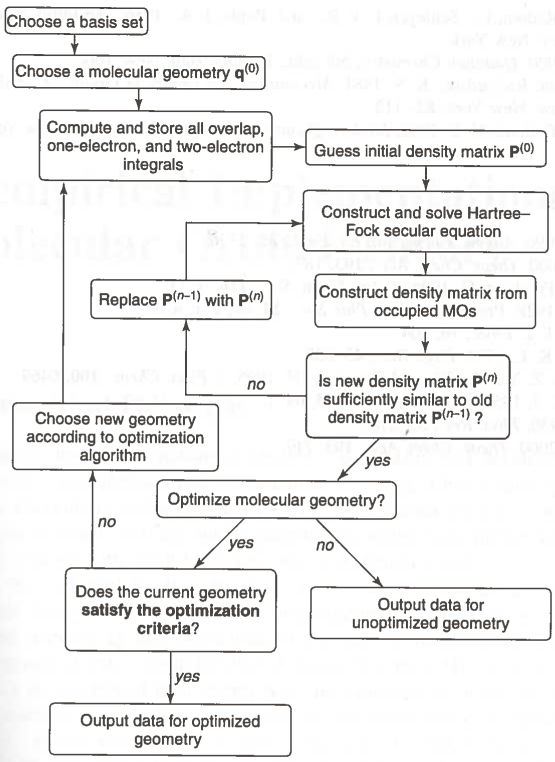
\includegraphics[width=\linewidth]{img/SCF.png}
  \caption{HF SCF procedure flowchart. Figure from \cite{Cramer:2004}}
  \label{fig:SCF}
\end{figure}

\subsection{\ac{DFT}}
The method outlined above employed an iterative procedure to calculate the coefficients
a a linear combination of basis functions describing the wave function of the
system, which is then used to calculate the energy of the system. We see that we
still need to calculate the repulsion potential between every electron. This is
simplified by using a density matrix to weight each of the basis that make up the
wave function of the other electrons.

Using a slightly different method, we calculate the energy directly as a functional
of the electron density distribution \cite{Sorland, Cramer:2004} described by
\begin{equation}\label{eq:densityintegral}
  \rho(\rvec) = n \int\abs{\Psi_e(\rvec, \rvec_1, \rvec_2,..., \rvec_n)} \text{d}\rvec_1\text{d}\rvec_2...\text{d}\rvec_n
\end{equation}
which is an integral over all the possible configurations of the electrons. The
coefficient $n$ is the total amount of electrons on the system. This method,
\ac{DFT}, allows to discard computing the wave function in the iterative process and
simply use the density instead.

The electron density has properties that are characteristic to each system, the
molecule,  it is constructed from. The first is that its integral over all space
is equal to the amount of electrons $n$ on the system \cite{Cramer:2004}
\begin{equation}
  \int_{\Real^3}\rho \text{d}\rvec = n
\end{equation}
The second is that the density has maxima on the positions of the nuclei, and
these maxima have the following value dependent on the nuclear charge of said
nuclei \cite{Cramer:2004}.
\begin{equation}
 \diff{\rvec}\rho(\rvec)\Bigg|_{\rvec = \Rvec_I} = -2Z_I\rho(\rvec)
\end{equation}

The energy is determined by a functional $E[\rho]$ made up of functionals representing
the kinetic energy of the electrons $T[\rho]$, the attraction potential $V_{Ne}[\rho]$,
and the two electron repulsion $V_{e}[\rho]$ \cite{Sorland, PhysRev.136.B864}
\begin{align}
  E[\rho] &= V[\rho] + T[\rho] + V_{e}[\rho]\\\label{eq:energyfunctional}
  T[\rho] &\equiv\braket{\rho(\rvec)| \frac{1}{2}\nabla^2| \rho(\rvec)} \\
  V_{e}[\rho] &\equiv \frac{1}{2}\braket{v_{e}(\rvec)| \rho(\rvec)}\\
  V_{Ne}[\rho] &= \braket{v_{Ne}(\rvec)|\rho(\rvec)}
\end{align}
Where the potential functions $v_{Ne}(\rvec)$  and $v_{e}(\rvec)$ are defined as the Coulomb
attraction between the electrons and the nuclei and the coulomb repulsion of the
density with itself \cite{Sorland} respectively.

The functional in Equation \ref{eq:energyfunctional} is not an appropiate approximation
of the energy, as we are assumming in the construction of $T[\rho]$ and $V_{e}[\rho]$
that the energy is known for the individual parts of the disconnected system \cite{Sorland}.
This means we are missing the exhchange-correlation contributions of the energy $E_{xc}{\rho}$.
With that in mind, the proper energy functional is shown as follows
\begin{equation}\label{eq:adjustedenergyfunc}
  E[\rho] = V[\rho] + T[\rho] + V_{e}[\rho] + E_{xc}[\rho]
\end{equation}

By the variational principle discussed previously, we are trying to minimize the energy
to get the best representation of the system with the given basis. Here we try to
find minima by differentiating \ref{eq:adjustedenergyfunc} with respect to $\rho$ giving us
\begin{align}\label{eq:energyderiv}
   \diff{\rho}E[\rho] = \diff{\rho}\left( V[\rho] + T[\rho] + V_{e}[\rho]\right) + V_{xc}
\end{align}
Where $V_{xc}$ is the functional derivative $\diff{\rho}E_{xc}[\rho]$ \cite{Cramer:2004}.
We can see that $V_{xc}$ seems to be a correction to the gradient to our first definition
of the the energy \ref{eq:energyfunctional}. The system described by Equation
\ref{eq:energyfunctional} is a system of non-interacting electrons. In this
system we can define one-electron operators $\hat{h}_i^{KS}$ as
\begin{align}
  \hat{h}_i^{KS} \phi_i &= \epsilon_i \phi_i \\
  \hat{h}_i^{KS} &= - \frac{1}{2}\nabla^2_i + v_{Ne} + \bra{\rho}v_e + V_{xc}
\end{align}
where $\phi$ are basis functions describing the function $\Psi$ from \ref{eq:densityintegral}
We can thus use $V_{xc}$ to iteratively minimize the energy in a systematic manner so we can
get the correct density for the system of interacting electrons \cite{Cramer:2004}.

This tells us that, given a set of basis functions $\phi$ describing
$\rho$ as defined in Equation \ref{eq:densityintegral}, we can compute the following
Kohn-Sham  matrix elements $\bar{K}_{\mu\nu}$ for a secular equation resembling that of the \ac{HF}
method. In this secular equation the elements $\bar{F}_{\mu\nu}$ are replaced by $\bar{K}_{\mu\nu}$.
\begin{equation}
  \bar{K}_{\mu\nu} = \braket{\phi_\mu|\left[- \frac{1}{2}\nabla^2_i + v_{Ne} + \bra{\rho}v_e + V_{xc}\right]|\phi_\nu}
\end{equation}
The rest of the procedure follows the same process as the \ac{SCF} explained on
the previous section.
What remains is to define $V_{xc}$ which can be represented in several ways by different methods
based on the basis functions used to construct the density, the reader is directed to
read on this in \cite{Cramer:2004} as this thesis will not delve deeper on the
matter.

\begin{acronym}
\acro{AUS}[\href{https://www.sigma2.no/content/advanced-user-support}{AUS}]{Numerical Methods in Quantum Chemistry}
\acro{BO}{Born-Oppenheimer}
\acro{CTCC}[\href{http://www.ctcc.no}{CTCC}]{Centre for Theoretical and Computational Chemistry}
\acro{DC}{Dielectric Continuum}
\acro{DFT}{Density Functional Theory}
\acro{EFP}{Effective Fragment Potential}
\acro{EU}{European Union}
\acro{HF}{Hartree-Fock}
\acro{Hylleraas}[\href{https://www.mn.uio.no/hylleraas/english/}{Hylleraas}]{Hylleraas
  Centre for Quantum Molecular Sciences}
\acro{HPC}{High Performance Computing}
\acro{KTH}{Royal Institute of Technology}
\acro{LDA}{Local Density Approximation}
\acro{MCD}{Magnetic Circular Dichroism}
\acro{MCSCF}{Multiconfiguration Self Consistent Field}
\acro{MM}{Molecular Mechanics}
\acro{MW}{Multiwavelet}
\acro{NFR}{Norwegian Research Council}
\acro{NMQC}[\href{http://www.ctcc.no/events/conferences/2015/numeric-conference/}{NMQC}]{Numerical Methods in Quantum Chemistry}
\acro{NOTUR}[\href{https://www.notur.no/}{NOTUR}]{Norwegian Metacenter for Computational Science}
\acro{PCM}{Polarizable Continuum Model}
\acro{PI}{Primcipal Investigator}
\acro{QC}{Quantum Chemistry}
\acro{QM}{Quantum Mechanics}
\acro{QM/MM}{Quantum Mechanics/Molecular Mechanics}
\acro{ROA}{Raman Optical Activity}
\acro{SC}{semiconductor}
\acro{SCF}{Self Consistent Field}
\acro{SHG}{Second Harmonic Genertation}
\acro{STSM}{Short-term scientific mission}
\acro{TPA}{Two-Photon Absorption}
\acro{WP}{Work Package}
\acro{CBS}{Complete Basis Set}
\acro{TCG}{Theoretical Chemistry Group}
\acro{vdW}{van der Waals}
\acro{SE}{Schrödinger Equation}
\acro{PES}{Potential Energy Surface}
\acro{LCAO}{Linear Combination of Atomic Orbitals}
\acro{MRA}{Multi-Resolution Analysis}
\acro{NS}{Nonstandard}
\end{acronym}

\biblio
\end{document}
